
%% Big Data Literary Review
%% 2015/08/26
%% by Will Hogan

\documentclass[10pt,journal,compsoc]{IEEEtran}
%
% If IEEEtran.cls has not been installed into the LaTeX system files,
% manually specify the path to it like:
% \documentclass[10pt,journal,compsoc]{../sty/IEEEtran}


% Some very useful LaTeX packages include:
% (uncomment the ones you want to load)


% *** MISC UTILITY PACKAGES ***
%
%\usepackage{ifpdf}
% Heiko Oberdiek's ifpdf.sty is very useful if you need conditional
% compilation based on whether the output is pdf or dvi.
% usage:
% \ifpdf
%   % pdf code
% \else
%   % dvi code
% \fi
% The latest version of ifpdf.sty can be obtained from:
% http://www.ctan.org/pkg/ifpdf
% Also, note that IEEEtran.cls V1.7 and later provides a builtin
% \ifCLASSINFOpdf conditional that works the same way.
% When switching from latex to pdflatex and vice-versa, the compiler may
% have to be run twice to clear warning/error messages.






% *** CITATION PACKAGES ***
%
\ifCLASSOPTIONcompsoc
  % IEEE Computer Society needs nocompress option
  % requires cite.sty v4.0 or later (November 2003)
  \usepackage[nocompress]{cite}
    \usepackage{romannum}
    \usepackage{tcolorbox}
    \usepackage{amsmath}
    \usepackage[noend]{algpseudocode}
    \usepackage[]{algorithm2e}
    \usepackage{tcolorbox}
    \usepackage{graphicx}
\else
  % normal IEEE
  \usepackage{cite}
\fi
% cite.sty was written by Donald Arseneau
% V1.6 and later of IEEEtran pre-defines the format of the cite.sty package
% \cite{} output to follow that of the IEEE. Loading the cite package will
% result in citation numbers being automatically sorted and properly
% "compressed/ranged". e.g., [1], [9], [2], [7], [5], [6] without using
% cite.sty will become [1], [2], [5]--[7], [9] using cite.sty. cite.sty's
% \cite will automatically add leading space, if needed. Use cite.sty's
% noadjust option (cite.sty V3.8 and later) if you want to turn this off
% such as if a citation ever needs to be enclosed in parenthesis.
% cite.sty is already installed on most LaTeX systems. Be sure and use
% version 5.0 (2009-03-20) and later if using hyperref.sty.
% The latest version can be obtained at:
% http://www.ctan.org/pkg/cite
% The documentation is contained in the cite.sty file itself.
%
% Note that some packages require special options to format as the Computer
% Society requires. In particular, Computer Society  papers do not use
% compressed citation ranges as is done in typical IEEE papers
% (e.g., [1]-[4]). Instead, they list every citation separately in order
% (e.g., [1], [2], [3], [4]). To get the latter we need to load the cite
% package with the nocompress option which is supported by cite.sty v4.0
% and later. Note also the use of a CLASSOPTION conditional provided by
% IEEEtran.cls V1.7 and later.




% *** GRAPHICS RELATED PACKAGES ***
%
\ifCLASSINFOpdf
  % \usepackage[pdftex]{graphicx}
  % declare the path(s) where your graphic files are
  % \graphicspath{{../pdf/}{../jpeg/}}
  % and their extensions so you won't have to specify these with
  % every instance of \includegraphics
  % \DeclareGraphicsExtensions{.pdf,.jpeg,.png}
\else
  % or other class option (dvipsone, dvipdf, if not using dvips). graphicx
  % will default to the driver specified in the system graphics.cfg if no
  % driver is specified.
  % \usepackage[dvips]{graphicx}
  % declare the path(s) where your graphic files are
  % \graphicspath{{../eps/}}
  % and their extensions so you won't have to specify these with
  % every instance of \includegraphics
  % \DeclareGraphicsExtensions{.eps}
\fi
% graphicx was written by David Carlisle and Sebastian Rahtz. It is
% required if you want graphics, photos, etc. graphicx.sty is already
% installed on most LaTeX systems. The latest version and documentation
% can be obtained at: 
% http://www.ctan.org/pkg/graphicx
% Another good source of documentation is "Using Imported Graphics in
% LaTeX2e" by Keith Reckdahl which can be found at:
% http://www.ctan.org/pkg/epslatex
%
% latex, and pdflatex in dvi mode, support graphics in encapsulated
% postscript (.eps) format. pdflatex in pdf mode supports graphics
% in .pdf, .jpeg, .png and .mps (metapost) formats. Users should ensure
% that all non-photo figures use a vector format (.eps, .pdf, .mps) and
% not a bitmapped formats (.jpeg, .png). The IEEE frowns on bitmapped formats
% which can result in "jaggedy"/blurry rendering of lines and letters as
% well as large increases in file sizes.
%
% You can find documentation about the pdfTeX application at:
% http://www.tug.org/applications/pdftex






% *** MATH PACKAGES ***
%
%\usepackage{amsmath}
% A popular package from the American Mathematical Society that provides
% many useful and powerful commands for dealing with mathematics.
%
% Note that the amsmath package sets \interdisplaylinepenalty to 10000
% thus preventing page breaks from occurring within multiline equations. Use:
%\interdisplaylinepenalty=2500
% after loading amsmath to restore such page breaks as IEEEtran.cls normally
% does. amsmath.sty is already installed on most LaTeX systems. The latest
% version and documentation can be obtained at:
% http://www.ctan.org/pkg/amsmath





% *** SPECIALIZED LIST PACKAGES ***
%
%\usepackage{algorithmic}
% algorithmic.sty was written by Peter Williams and Rogerio Brito.
% This package provides an algorithmic environment fo describing algorithms.
% You can use the algorithmic environment in-text or within a figure
% environment to provide for a floating algorithm. Do NOT use the algorithm
% floating environment provided by algorithm.sty (by the same authors) or
% algorithm2e.sty (by Christophe Fiorio) as the IEEE does not use dedicated
% algorithm float types and packages that provide these will not provide
% correct IEEE style captions. The latest version and documentation of
% algorithmic.sty can be obtained at:
% http://www.ctan.org/pkg/algorithms
% Also of interest may be the (relatively newer and more customizable)
% algorithmicx.sty package by Szasz Janos:
% http://www.ctan.org/pkg/algorithmicx




% *** ALIGNMENT PACKAGES ***
%
%\usepackage{array}
% Frank Mittelbach's and David Carlisle's array.sty patches and improves
% the standard LaTeX2e array and tabular environments to provide better
% appearance and additional user controls. As the default LaTeX2e table
% generation code is lacking to the point of almost being broken with
% respect to the quality of the end results, all users are strongly
% advised to use an enhanced (at the very least that provided by array.sty)
% set of table tools. array.sty is already installed on most systems. The
% latest version and documentation can be obtained at:
% http://www.ctan.org/pkg/array


% IEEEtran contains the IEEEeqnarray family of commands that can be used to
% generate multiline equations as well as matrices, tables, etc., of high
% quality.




% *** SUBFIGURE PACKAGES ***
%\ifCLASSOPTIONcompsoc
%  \usepackage[caption=false,font=footnotesize,labelfont=sf,textfont=sf]{subfig}
%\else
%  \usepackage[caption=false,font=footnotesize]{subfig}
%\fi
% subfig.sty, written by Steven Douglas Cochran, is the modern replacement
% for subfigure.sty, the latter of which is no longer maintained and is
% incompatible with some LaTeX packages including fixltx2e. However,
% subfig.sty requires and automatically loads Axel Sommerfeldt's caption.sty
% which will override IEEEtran.cls' handling of captions and this will result
% in non-IEEE style figure/table captions. To prevent this problem, be sure
% and invoke subfig.sty's "caption=false" package option (available since
% subfig.sty version 1.3, 2005/06/28) as this is will preserve IEEEtran.cls
% handling of captions.
% Note that the Computer Society format requires a sans serif font rather
% than the serif font used in traditional IEEE formatting and thus the need
% to invoke different subfig.sty package options depending on whether
% compsoc mode has been enabled.
%
% The latest version and documentation of subfig.sty can be obtained at:
% http://www.ctan.org/pkg/subfig




% *** FLOAT PACKAGES ***
%
%\usepackage{fixltx2e}
% fixltx2e, the successor to the earlier fix2col.sty, was written by
% Frank Mittelbach and David Carlisle. This package corrects a few problems
% in the LaTeX2e kernel, the most notable of which is that in current
% LaTeX2e releases, the ordering of single and double column floats is not
% guaranteed to be preserved. Thus, an unpatched LaTeX2e can allow a
% single column figure to be placed prior to an earlier double column
% figure.
% Be aware that LaTeX2e kernels dated 2015 and later have fixltx2e.sty's
% corrections already built into the system in which case a warning will
% be issued if an attempt is made to load fixltx2e.sty as it is no longer
% needed.
% The latest version and documentation can be found at:
% http://www.ctan.org/pkg/fixltx2e


%\usepackage{stfloats}
% stfloats.sty was written by Sigitas Tolusis. This package gives LaTeX2e
% the ability to do double column floats at the bottom of the page as well
% as the top. (e.g., "\begin{figure*}[!b]" is not normally possible in
% LaTeX2e). It also provides a command:
%\fnbelowfloat
% to enable the placement of footnotes below bottom floats (the standard
% LaTeX2e kernel puts them above bottom floats). This is an invasive package
% which rewrites many portions of the LaTeX2e float routines. It may not work
% with other packages that modify the LaTeX2e float routines. The latest
% version and documentation can be obtained at:
% http://www.ctan.org/pkg/stfloats
% Do not use the stfloats baselinefloat ability as the IEEE does not allow
% \baselineskip to stretch. Authors submitting work to the IEEE should note
% that the IEEE rarely uses double column equations and that authors should try
% to avoid such use. Do not be tempted to use the cuted.sty or midfloat.sty
% packages (also by Sigitas Tolusis) as the IEEE does not format its papers in
% such ways.
% Do not attempt to use stfloats with fixltx2e as they are incompatible.
% Instead, use Morten Hogholm'a dblfloatfix which combines the features
% of both fixltx2e and stfloats:
%
% \usepackage{dblfloatfix}
% The latest version can be found at:
% http://www.ctan.org/pkg/dblfloatfix




%\ifCLASSOPTIONcaptionsoff
%  \usepackage[nomarkers]{endfloat}
% \let\MYoriglatexcaption\caption
% \renewcommand{\caption}[2][\relax]{\MYoriglatexcaption[#2]{#2}}
%\fi
% endfloat.sty was written by James Darrell McCauley, Jeff Goldberg and 
% Axel Sommerfeldt. This package may be useful when used in conjunction with 
% IEEEtran.cls'  captionsoff option. Some IEEE journals/societies require that

\hyphenation{op-tical net-works semi-conduc-tor}
%\graphicspath{ {C:\Users\william\Downloads\Latex\BigData_LitReview} }

\begin{document}

\title{Big Data}

\author{Will~Hogan 
	\\{4th Year Software Development}
	\\{Research Methodologies in Computing and I.T.}}

% for Computer Society papers, we must declare the abstract and index terms
% PRIOR to the title within the \IEEEtitleabstractindextext IEEEtran

\IEEEtitleabstractindextext{%
\begin{abstract}
In modern day computing, the term Big Data has become increasingly popular and equally significant. In a nutshell, it's a term that's used to describe large amounts of data. This Data is being created and stored on a massive scale globally. The purpose of this literary review is to delve into the world of Big Data and ascertain where it's used, why organisations want it and where it fits into our modern day society. 
\end{abstract}}


\maketitle

\IEEEdisplaynontitleabstractindextext

\IEEEpeerreviewmaketitle

\IEEEraisesectionheading{\section{Introduction}\label{sec:introduction}}

\IEEEPARstart{W}{e} live in an ever changing world and technology is one of the things that's moving quickly. There are millions of devices globally that are storing, sending and receiving large amounts of data and there are multiple reports suggesting that the rate of data creation will continue to grow at a rate between 40 and 60\% a year[1]. IBM have stated that there are 2.5 quintillion bytes of data created every day and that the last two years has seen 90\% of the worlds data created[2]. This data is being created by a number of different devices and sources, for example mobile phones that are so much more than call making devices. The University of cambridge suggest that by 2020, 80\% of the worlds population will own a mobile phone[3]. With these predictions and statistics, it's fair to say that data creation will continue to increase. Social media has seen a dramatic increase in usage, reports suggest that Facebook are dealing with a billion content information queries per day[4]. But it's not just Social Media that's creating large amounts of data, Netflix are accumulating billions of viewer ratings, with members searching and adding millions of items each day[4]. It's also worth highlighting that with these increases in data creation / production, there will inevitably be an increase in Data related positions and careers. The UK government have reported that they predict an increase in demand for Big Data staff of between 13 and 23\% between now and 2017[5]. To add further to this domino effect, it's important to mention that data needs to be stored somewhere if it's going to be of any use and i'm not just talking about excel spreadsheets or traditional databases methods, but something that works on a much larger scale, that can deal with the vast amounts of data and information being circulated globally. This increase creates a need for better software to handle the data, bigger and better servers to store it and more staff to operate them. 

% You must have at least 2 lines in the paragraph with the drop letter
% (should never be an issue)


\subsection{A Comprehensive look at Data}
The term Big Data has been around for a number of years, but it's really become more relevant with the increase in Social Media usage, contributed to by big names like Facebook, Twitter and Instagram, but if we look in more depth at what data actually is we can gain a more insightful perspective, which in turn will help to understand how data works. Essentially if we break any type of data down to it's most raw component, data in technological terms is simply just a collection of 1's and 0's that form binary code. Humans have mapped binary code into the more human readable form, which is known as the ASCII(American Standard Code for Information Interchange) character encoding standard[6]. This standard contains all the letters of the alphabet and their equivalent binary values and as we put letters and sentences together it's worth noting that there will always be a binary representation at the lowest level. Data can be structured or unstructured, with structured there are specific dataypes ie integers, strings and Floats. From a Relational database model the structured data may also be normalised. On the flipside unstructured data is pure raw data and doesn't necessarily comply with any format or type. As time has moved on and technology has advanced, it's hard to think of things in terms of bits and bytes, however in the world of Big Data, the words Pettabytes, Exabytes, Zettabytes and even Yottabytes are becoming common place. To help put this into perspective, consider the following information taken from the School of Information Management and Systems, Berkeley University in 2003[7];\\\\\\
\begin{tabular}{lp{0.33\textwidth}r}
	\bfseries Data Size & \bfseries Example &
	\bfseries  \\[1ex]
	100 Kilobytes & A low resolution photo. \\
	5 Megabytes & The complete works of Shakespeare. \\
	100 Gigabytes & A library floor of academic journals. \\
	10 Terabytes & Print collections of the U.S. Lib. of Congress. \\
	200 Petabytes & All printed material. \\
	2 Exabytes & Total volume of information generated in 1999
\end{tabular}\\\\\\
With these statistics in mind, we can build a picture as to how big big data can actually get, bearing in mind the fact that this paper was written thirteen years ago. As the years have elapsed, data has grown exponentially and with that comes new terminologies and buzz words that fit specific circumstances. As detailed by Doug Laney[8], who outlines a well-known definition(also called 3Vs) to explain this. Volume, velocity, and variety. The definition of 3Vs implies that the data size is large, the data will be created rapidly, and the data will exist as multiple types and captured from different sources, respectively.

\subsection{Big Data Analytics}
Big Data analytics is a combination of Big Data and Analytics. But firstly just for clarification purposes, let us define what exactly Data Analytics is. Data analytics is the science of scrutinising raw data with the hope of discovering trends or habits in specific business areas. It's important to note that Fayyad and his colleagues mentioned back in 1996, that due to the emerging field of Knowledge Discovery in Databases(KDD), that there was an urgent need for new computational tools and theories to aid humans in discovering new and useful information[8]. Furthermore if we fast forward to 2009, a survey from the TDWI(transforming data into intelligence), revealed that 35\% of Organisations have reported practicing some form of advanced analytics, whereas 85\% explained that they would be practicing it within the next 3 years[9]. Based on this, it seems that Fayyad and his colleagues were spot on the mark and while it's important to acknowledge there foresight, it's also equally important to ask the question why this happened? Change is something that happens in many different environments, business being just one. But analytics itself hasn't just helped to assess situations, it has helped us discover what has changed, it's then with these discoveries that we can react accordingly and make the right decisions[10]. To add to this, it's worth noting that companies and organisations opted to use Data Analytics as a chance to beat the worldwide recession and help build a path to recovery[10].

\subsubsection{Data Mining} 
One of the methods that organisations can use in order to benefit from analysing their data, is Data Mining. To quote Oracle;

\textbf{\textit{"Data mining is the practice of automatically searching large stores of data to discover patterns and trends that go beyond simple analysis."}}[11]. 

Let's explore this a bit further. Fig. 1 outlines what most Data mining algorithms contain, initialisation, data input, data scan, rules construction and also rules update operators[12].\\

\newtcolorbox{algoBox}[1]
{colback=white!5!white,colframe=white!25!black,fonttitle=\bfseries,title=#1}

\begin{algoBox}{\textbf{Figure 1: Data Mining Algorithm}}
	{Input data \textit{D}}\\
	{Initialize candidate solutions \textit{r}}\\
	\While{the termination criterion is not met}
	{
		\textit{d = Scan(D);\\
			v = Construct(d, r, o);\\
			r = Update(v);}
	}
	Output rules \textit{r};
\end{algoBox}

Lets break this down piece by piece in order to understand it better. \textit{D} is the actual raw data, \textit{d} is the data entered in by the scan operator, \textit{r} are the rules, \textit{o} are the predefined measurement and \textit{v} the candidate rules. The scan, construct and update operators will continue to loop until the search criteria have been met.
There are different methods used in Data Mining, in Fig 2. we see another method used called Clustering. With this method data can be seperated into different labelled groups using \textit{k-means}[13].\\


\begin{algoBox}{\textbf{Figure 2: \textit{k-means} Algorithm}}
	{Input data \textit{D}}\\
	{Randomly create a set of centroids \textit{c}}\\
	\While{the termination criterion is not met}
	{
		\textit{v = Assign(D, c);\\
			c = Update(v);}
	}
	Output centroids \textit{c};
\end{algoBox}

To detail what's happening in the above, firstly we create a random set of Centroids, these centroids represent the patterns created by user input are divided into specific groups[14]. After this, the assignment operator checks the distance between the centroids and the patterns in order to ascertain which group each pattern belongs too. The formula used to calculate this(1) can be written as so;

\begin{equation}
	SSE = \sum_{i=1}^{k} \sum_{j=1}^{n_i} D( x_{ij} - c_i)
\end{equation}

Where SSE is the squared sum of errors, which is used to measure cohesion of the data mining results. In the above formula \textit{k} is entered by the user; ni the number of
data in the ith cluster; \textit{xij} the \textit{j}th datum in the \textit{i}th cluster; \textit{ci} is the mean of the \textit{i}th cluster; [14]. 

With Data Mining, the most common method to measure distance is the Euclidean distance, defined as

\begin{equation}
\mathbf{D(p_{i}, p_{j})} = 
\left(
\sum_{l=1}^{d} |p_{il}, p_{jl}|^2
\right)^{1/2}
\end{equation}

Where \textit{pi} and \textit{pj} are the positions of two different pieces of data.

\subsubsection{Data Warehousing}
Like the buzz words Big Data and Data Mining, Data Warehousing is another term that's being widely used in the world of Data Analytics. Essentially a Data Warehouse is a large scale database that stores data. But it's what it stores that defines it and sets it apart from other databases. Oracle have stated that it's a Relational Database that's not designed for transaction purposes, but more for querying and Analysis[15]. To put this into perspective, You might be looking to see trends, spikes and customer spending as apposed to searching a database for when a particular employee started in a given organisation. To enable this sort of broad scale searching and analysis, several databases from different sections of an organisation, feed into the Data Warehousing which essentially stores everything that's being sent to it. From here, the data can be split and seperated into department specific databases known as Data Marts. The method used to get to this point is called ETL(Extraction, Transformation and Loading). Extraction means retrieve the data from the various Database sources, Transformation is turning that data into something useful and Loading refers to the process of saving the data to the Data Warehouse, illustrated in Fig. 3[15].\\

\textbf{Figure 3: Data Warehousing Example}
\begin{figure}[ht!]
	\centering
	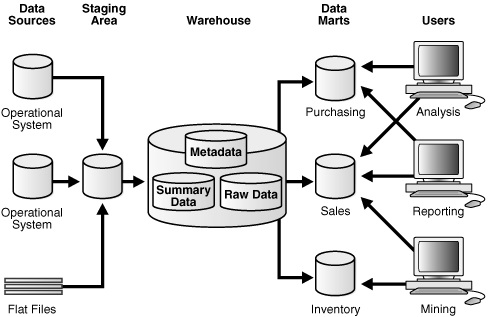
\includegraphics[width=88mm]{dwarehouse.jpg}
\end{figure}

This type of concept may seem convoluted to the average client, but what will make sense is how it will affect their organisations financially. Inmon states[16], that Data Warehousing significantly reduces the cost of information, with the result that organisations that use a Data Warehouse, can access a specific piece of information for \$100, as apposed to an organisation that doesn't have a Data Warehouse, who will access the same piece of information for \$10,000. 

\subsection{The Importance of Big Data}

\subsection{Big Data, the next steps}
Mention about "Spark", the new Paradigm [A survey on platforms for big data analytics]

\section{Conclusion}

\begin{thebibliography}{1}

\bibitem{IEEEhowto}
OECD (2013) New sources of growth- knowledge based capital. OECD, Paris. 
http://www.oecd.org/sti/inno/knowledge-based-capital-synthesis.pdf.

\bibitem{IEEEhowto}
Harness the Power of Big Data The IBM Big Data Platform
https://www-01.ibm.com/software/data/bigdata/what-is-big-data.html

\bibitem{IEEEhowto}
http://www.cam.ac.uk/research/discussion/talkin-bout-a-revolution-how-to-make-the-digital-world-work-for-us

\bibitem{ITEEEhowto}
Amatriain X (2013) Beyond Data: from user information to business value through personalized recommendations
and consumer science, CIKM’13. San Francisco, CA, USA

\bibitem{IEEEhowto}
Seizing the data opportunity: A strategy for UK data capability
bis-13-1250-strategy-for-uk-data-capability-v4.pdf

\bibitem{IEEEhowto}
http://www.asciitable.com

\bibitem{IEEEhowto}
How Much data.pdf
Release date: October 27, 2003. © 2003 Regents of the University of California

\bibitem{IEEEhowto}
Fayyad UM, Piatetsky-Shapiro G, Smyth P. From data mining to knowledge discovery in databases. AI Mag.1996

\bibitem{IEEEhowto}
TDWI Best Practices Report Next Generation Data Warehouse Platforms (Q4 2009), available on tdwi.org.

\bibitem{IEEEhowto}
Big Data Analytics by Philip Russom 2011
http://www.sas.com/content/dam/SAS/en\_us/doc/research2/big-data-analytics-105425.pdf

\bibitem{IEEEhowto}
https://docs.oracle.com/cd/B28359\_01/datamine.111/b28129/process.htm

\bibitem{IEEEhowto}
Tsai C-W, Lai C-F, Chiang M-C, Yang L. Data mining for internet of things: a survey. IEEE Commun Surveys Tutor.
2014;16

\bibitem{IEEEhowto}
SOME METHODS FOR CLASSIFICATION AND ANALYSIS OF MULTIVARIATE OBSERVATIONS by J Macqueen, University of California
https://pdfs.semanticscholar.org/a718/b85520bea702533ca9a5954c33576fd162b0.pdf

\bibitem{IEEEhowto}
Krishna K, Murty MN. Genetic k-means algorithm. IEEE Trans Syst Man Cyber Part B Cyber. 1999;

\bibitem{IEEEhowto}
https://docs.oracle.com/cd/B10500\_01/server.920/a96520/concept.htm

\bibitem{IEEEhowto}
Building the Data Warehouse Third Edition, W.H.Inmon, 2002


\end{thebibliography}

\end{document}
